\documentclass[12pt, a4paper] {article}
\usepackage[utf8]{inputenc}
\usepackage{graphicx}
\usepackage{indentfirst}

\begin{document}
	\begin{titlepage}
    \vspace*{\stretch{1.0}}
	\begin{center}
		\Large\textbf{Instalação Arch Linux!}\\
		\large\textit{Victor Emanuel Almeida}
  \end{center}
	 	 \vspace*{\stretch{2.0}}
		\begin{figure}[htb]
			\centering
			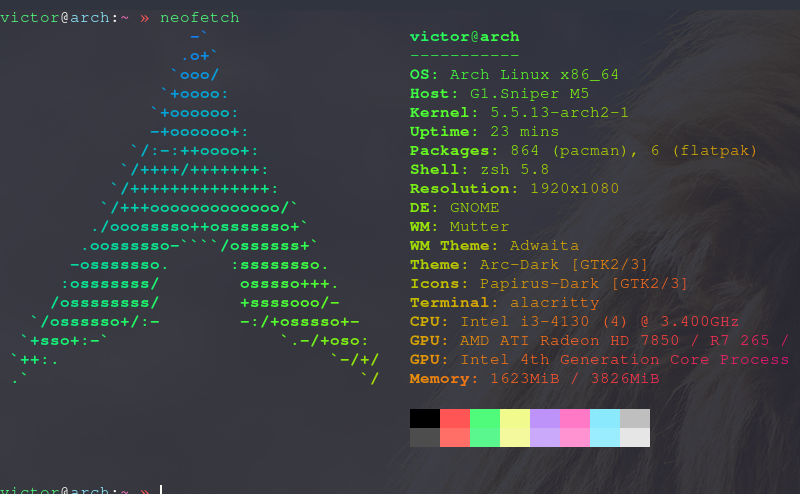
\includegraphics[width=\linewidth]{images/Simbolo.png}
			\caption{Imagem do Simbolo do Arch Linux saido do neofetch}
			\label{fig:neofetch}
		\end{figure}
		\end{titlepage}
	
	\section{Passo: Conectar na internet, no caso via wifi.}
		
	No meu notebook da lenovo, o hardware utilizado para conectar no wifi vinha bloqueado, para saber se isso esta acontecendo utilize:\\
	 	\textbf{$\ast$rfkill list all$\ast$}. Veja como fica o OUTPUT:
		\begin{figure}[htb]
			\centering
			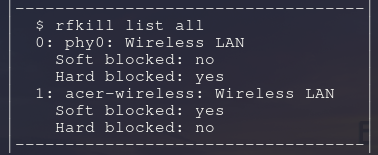
\includegraphics[width=\linewidth]{images/1.png}
			\caption{Imagem do output do comando rfkill list all}
			\label{fig:rfkill}
		\end{figure}

		Tendo a certeza que esta desbloqueado, basta usar \textbf{$\ast$wifi-menu$\ast$}, e então será aberta uma tela na qual basta selecionar a rede (aparecera todos os SSID disponiveis para conectar), e informar a senha.\\
		\begin{figure}[htb]
			\centering
			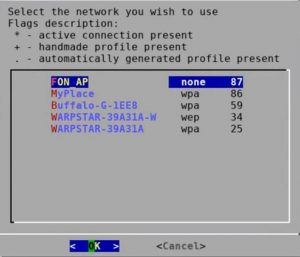
\includegraphics[width=75mm]{images/wifi-menu.jpg}
			\caption{Imagem do comando wifi-menu}
			\label{fig:Wifi-menu}
		\end{figure}

	\section{Passo: Particionar o Disco.}

	Primeiramente é sempre bom verificar as partições já existentes no disco, para fazer isso vamos usar \textbf{$\ast$fdisk -l$\ast$}, o parametro (-l) é para listar todas as partições existentes.

	Agora sabendo qual o disco a ser particionado e as partições já existentes basta utilizar \textbf{$\ast$cfdisk /dev/sdx$\ast$}. Obs: no lugar de (x) coloque a letra correta para indicar seu disco, se for o disco primario sera ``sda'', mas pode ser sdb, sdc, etc \ldots

	Para usar o cfdisk é muito simples basta usar as setas para navegar até o (new), digitar o tamanho da particao e selecionar o tipo dela. Essa é a tela que vc vai encontrar:
	\begin{figure}[htb]
    \centering
    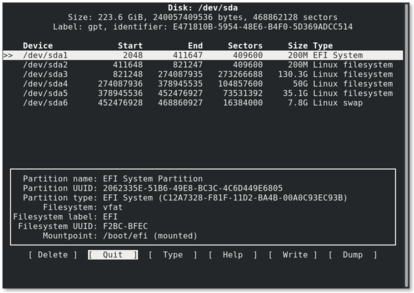
\includegraphics[width=\linewidth]{images/cfdisk.png}
    \caption{Imagem do output do comando cfdisk}
		\label{fig:cfdisk}
  \end{figure}

	Quando se instala o Arch, recomenda-se fazer 4 partições. Sendo elas:\\
	\centering\textbf{``/boot''|``/''|``/home''|``swap''}

\end{document}
